
\chapter{Introduction}\label{ch:introduction}

\section{Introduction}
The success of machine-readable data on the web can be seen with the rate of adoption from webmasters. From a sample of 3.2 billion web pages in 2017 \cite{webDataCommons2017}, 38.9\% contained machine-readable data. This is up from 30\% in 2014 \cite{webDataCommons2014} from 2 billion web pages. With the excess number of machine-readable data formats and the markup vocabularies available, webmasters have the difficulty of choosing which format and vocabulary to use. 

As each machine-readable data format has their own advantages and disadvantages, webmasters have the difficulty in choosing which format and subsequently which vocabulary best suits their needs. Schema.org aims to make it easier for webmasters by providing a single vocabulary \cite{schemaOrg} for the following machine-readable formats: RDFa; Microdata; and JSON-LD. Although Schema.org's vocabulary is extensive it relies on extensions to provide terms in areas that are lacking \cite{schemaExtensions}. 

Section \ref{sec:schema} describes how properties and types are linked through a single hierarchy. However, due to the extensive number of properties each type can have, webmasters have a difficult time choosing which properties to include. Profiles like Google Dataset Search and Bioschemas aim to help by recommending and suggesting properties that webmasters should include when marking up resources. Bioschemas goes one step further and enhances the Schema.org model by providing an additional layer of constraints (marginality, cardinality and controlled vocabularies)\cite{gray2017bioschemas}. Additionally, Bioschemas aims to recommend 6 properties in a type to users in order to get the best result possible in discovery searches.

\newpage
Although there exists many systems to help users generate Schema.org markups, from my research all systems found are limited to a small selection of types. The Bioschemas community are interested in a reconfigurable system which takes a declarative description of a Bioschemas specification and dynamically generates a form to help users create their markup. This is due to Bioschemas rapidly evolving, so ultimately needs a system that is able to keep up with new profiles and types.

\section{Aim \& Objectives}
The aim of this project is to develop a system to support users in the creation of Bioschemas markup for their web resources.

\noindent
The aim will be met through the following objectives:
\begin {enumerate}
    \item Review existing tools for generating and validating Schema.org markup.   
    \item Allow users to easily generate Bioschemas markup through an intuitive and aesthetically pleasing user interface.
    \item To evaluate the final system's usefulness and validate that the generated data is syntactically correct and compliant with the Bioschemas.org specifications.
\end{enumerate}

\chapter{Background}
\section{Introduction}
The aim of this project is to develop a system that helps generate markup based on the specifications from Bioschemas.org and subsequently Schema.org. The structured data produced from the system should be in a format that is widely supported and usable on the web. This chapter will explore the topics relevant to the system and its requirements: machine-readable data; Schema.org; profiles over Schema.org; and existing tools for creating and validating Schema.org markups will be reviewed.

\section{Machine-readable Data}
Machine-readable data is structured data that is in a format that can be easily processed by a machine and can be categorised into two types: Human-readable data and Data file formats. Human-readable data is marked up in a way that can be read and understood by humans but also by machines (e.g microformats and RDFa). Data file formats on the other hand is more complex and is intended to only be processed by machines (e.g RDF and JSON-LD). \newline

\subsection{Machine-readable Data on the Web}
\label{sec:machinereadable}
Before machine-readable data was introduced to the web, applications that utilised underlying data on web pages had to use custom data extractors to convert the plain HTML into machine-readable data. These extractors were difficult to implement and were prone to breaking when a website changed its layout \cite{guha2016schema}. By adding machine-readable data to the web it made it easier for applications and webmasters to create and read machine-readable data, enabling search engines to interpret the contents of the web page reliably. This gives users a more rich and interactive experience through features such as Google Rich Snippets\footnote{\url{https://developers.google.com/search/docs/guides/mark-up-content} (accessed 3/11/18)} and Knowledge Graph\footnote{\url{https://developers.google.com/knowledge-graph/} (accessed 3/11/18)}. In the following subsections I will discuss the four main formats of machine-readable data on the web:\newline

{\setstretch{1.0}
\begin{enumerate}
    \item Microformats
    \item RDFa
    \item HTML Microdata 
    \item JSON-LD 
\end{enumerate}
}

\subsubsection{Microformats}
Introduced in 2005 \cite{microformasIntroduction}, Microformats was the first approach to introduce machine-readable data to the web. Using HTML/XHTML standards, microformats adds metadata into the markups tags, this is indicated by the following attributes: \texttt{class}, \texttt{rel} and \texttt{rev}. This allows applications to easily extract and process information on a web page without the need for custom extraction tools (mentioned in  Section \ref{sec:machinereadable}). 

Many varieties of microformats were developed to describe particular types of information such as events, news or products. However, only hCalander \cite{hcalanderMicroformat} and hCard \cite{hcardMicroformat} were formally published, with the others remaining as drafts.

\newpage
Although microformats are simple and easy to use, they come with limitations. One limitation is that microformats have issues with scoping \cite{microformatsIssues}. Meaning if one type overlaps another, microformats does not have a way to identify which properties belongs to which type. Another limitation is name spacing \cite{microformatsIssues}. Different microformats may use the same property name, leading to ambiguity of the property definitions. With these limitations and the numerous formats available it can become confusing for the webmasters \cite{schemaOrg}. Therefore, webmasters have begun to favour new and more advanced machine-readable formats. 

The hCard example shown in Listing \ref{lst:hCard} represents a person. The HTML element \texttt{link} specifies which type of microformat is used through the attribute \texttt{href}, in this case hCard. The \texttt{span} element with the attribute \texttt{class="fn"} was used to specify the person's full name of \say{John Doe}. The \texttt{img} element with attribute \texttt{class="photo"} was used to specify a photo of the person, \say{johndoe.jpg}. Finally, the \texttt{a} element with attribute \texttt{class="url"} was used to specify the homepage for this person, \say{http://www.johndoe.com} \cite{hcardMicroformat}.\newline

\noindent
\textbf{hCard Example:}
{\setstretch{1.0}
\begin{lstlisting}[language=HTML,caption={A hCard example},captionpos=b,label={lst:hCard}]
<link rel="profile" href="http://microformats.org/profile/hcard" />
    <div class="vcard">
        <span class="fn">John Doe</span>
        <img class="photo" src="johndoe.jpg"/>
        John's Website: 
        <a class="url" href="http://www.johndoe.com">johndoe.com</a>
    </div>
</div>
\end{lstlisting}
}

\subsubsection{RDFa}
RDFa (Resource Description Framework in attributes) is a human-readable markup of RDF. It allows webmasters to add machine-readable data to XHTML, XML or SVG by adding the ability to write RDF triples as attribute values \cite{sikos2015mastering}. There are currently 4 versions of RDFa: 

{\setstretch{1.0}
\begin{enumerate}
    \item RDFa Lite 1.1 (A small subset of RDFa for simple to moderate complexity of structured data) \cite{sporny2015rdfa}
    \item HTML+RDFa 1.1 (Adapting RDFa Core 1.1 and RDFa Lite 1.1 specifications for use in HTML5 and XHTML5) \cite{mccarron2013html+}
    \item RDFa Core 1.1 (Specification for attributes to express structured data in any markup language) \cite{adida2007rdfa}
    \item XHTML+RDFa 1.1  (Defined attributes and syntax for embedding semantic markup in XHTML)
    \cite{adida2008rdfa}
\end{enumerate}
}

\newpage
The advantage of RDFa compared to microformats, is that RDFa has the ability to declare the name space of the of the property. This eliminates any ambiguity of the property. RDFa also allows the use of more than one vocabulary. This aids webmasters in describing information that may not covered in certain vocabularies. 

The RDFa example shown in Listing \ref{lst:rdfa} represents a person. The element \texttt{p} specifies the vocabulary used with attribute \texttt{vocab}, in this case Schema.org. It also specifies the type of property is being described, a Person, through the \texttt{typeof} attribute. The \texttt{span} element with the attribute \texttt{property="name"} was used to specify the person's name of \say{John Doe}. The \texttt{img} element with attribute \texttt{property="image"} was used to specify a photo of the person, \say{johndoe.jpg}. Finally, the \texttt{a} element with attribute \texttt{property="url"} was used to specify the URL for this person, \say{http://www.johndoe.com}.\newline

\noindent
\textbf{RDFa Example:}
{\setstretch{1.0}
\begin{lstlisting}[language=HTML,caption={A RDFa Example},captionpos=b,label={lst:rdfa},showstringspaces=false]
<p vocab="http://schema.org/" typeof="Person">
    <span property="name">John Doe</span>
    <img src="johndoe.jpg" alt="John Doe" property="image" />
    John's web site: 
    <a property="url" href="http://www.johndoe.com">johndoe.com</a>
</p>
\end{lstlisting}
}

\subsubsection{HTML Microdata}
HTML Microdata is defined as a \say{HTML extension that defines new HTML attributes to embed simple machine-readable data in HTML documents} \cite{htmlMicrodata2018}. HTML microdata represents machine-readable data as a group of name-value pairs \cite{sikos2015mastering} where groups are called items, and each name-value pair is a property. 

The main advantage of HTML microdata is that it is simple for webmasters to learn and process \cite{htmlMicrodata2018}, but due to its simplicity it has limitations. Limitations of HTML microdata include: only supporting two data types (strings and URLs), not retaining markup structure and not preserving internationalisation-related information except when encoded as microdata \cite{htmlMicrodata2018}. The World Wide Web Consortium (W3C) is a international community, that develops protocols and guidelines for the web to ensure long-term growth \cite{w3cFAQ}. W3C currently recommends webmasters to choose JSON-LD or RDFa over HTML microdata \cite{htmlMicrodata2018} if they need to support the limitations previously discussed. 

\newpage
The Microdata example shown in Listing \ref{lst:micro} represents a Person. The \texttt{div} element specifies the property type and vocabulary through the attribute \texttt{itemtype}, in this example the vocabulary is Schema.org and is of type Person.  The \texttt{span} element with the attribute \texttt{itemprop="name"} was used to specify the person's name of \say{John Doe}. The \texttt{img} element with attribute \texttt{itemprop="image"} was used to specify a photo of the person, \say{johndoe.jpg}. Finally, the \texttt{a} element with attribute \texttt{itemprop="url"} was used to specify the URL for this person, \say{http://www.johndoe.com}.\newline


\noindent
\textbf{Microdata Example:}
{\setstretch{1.0}
\begin{lstlisting}[language=HTML,caption={A Microdata Example},captionpos=b,label={lst:micro},showstringspaces=false]
<div itemscope="itemscope" itemtype="http://schema.org/Person">
    <span itemprop="name">John Doe</span>
    <img src="johndoe.jpg" alt="John Joe" itemprop="image" />
    John's web site:
    <a href="htp://www.johndoe.com" itemprop="url">johndoe.com</a>
</div>
\end{lstlisting}
}

\subsubsection{JSON-LD}\label{sec:jsonld}
The latest machine-readable data format introduced for the web was JSON-LD (JavaScript Object Notation for Linked Data). Unlike other web formats JSON-LD is "described as JavaScript code rather than markup elements and attributes" \cite{sikos2015mastering}, meaning that JSON-LD is completely detached from the HTML code. 

Due to JSON-LD being in a human-readable format, it is easy for webmasters to create and read the data without the aid of any tools. With JSON-LD being separate from the markup, it can be easily reused and interchanged without having to edit the markup. However, the disadvantage to this is that if the webmaster changes the content of web page they may forget to update the JSON-LD capturing this change. 

The JSON-LD example shown in Listing \ref{lst:jsonld} represents a person. The key value pair \texttt{@context} specifies the vocabulary being used, in this case it is Schema.org. The key value pair \texttt{@type} is used to specify the property type from the specified vocabulary, in this case it is Person. The key value pair \texttt{name} specifies the name of the person. The key value pair \texttt{image} was used to specify a photo of the person. Finally, the key value pair \texttt{url} specifies the URL of the person.
\newline

\newpage
\noindent
\textbf{JSON-LD Example:}
{\setstretch{1.0}
\begin{lstlisting}[language=HTML,caption={A JSON-LD Example},captionpos=b,label={lst:jsonld},showstringspaces=false]
<script type="application/ld+json">
{
    "@context":"http://schema.org",
    "@type":"Person",
    "name":"John Doe",
    "image":"johndoe.jpg",
    "url":"http://www.johndoe.com"
}
</script>
\end{lstlisting}
}

\subsubsection{Adoption Statistics}
The Web Data Commons project \cite{webDataCommons} extracts machine-readable structured data from the Common Crawl \cite{commonCrawlWeb}, the largest copy of the web publicly available. The project provides statistics on the formats of structured data used on the web from 2009 onwards. \newline

\begin{table}[h!]
\centering
\begin{tabular}{ |p{4cm}|R{2.5cm}|R{2.5cm}|}
 \hline
 Format & Domains 2017 & Domains 2016 \\
 \hline
 HTML Microdata & 3,743,822 & 2,537,539 \\
 Microformats (hCard) & 2,758,884 & 1,668,039  \\
 JSON-LD & 2,685,738 & 2,116,755\\
 RDFa & 1,209,430 & 938,830 \\
 \hline
\end{tabular}
\caption{Top 4 used machine-readable data formats from 2016/2017 Common Crawl \cite{webDataCommons2017,webDataCommons2016}}
\label{table:1}
\end{table}

Table \ref{table:1} shows the significant growth of machine-readable data on the web over the course of a year between 2016 and 2017. This growth is due to more companies supporting and utilising machine-readable data on the web. For example, during this time Google implemented Rich Cards\footnote{\url{https://webmasters.googleblog.com/2016/05/introducing-rich-cards.html} (accessed 21/11/2018)} and both Google\footnote{\url{https://www.seroundtable.com/google-news-fact-check-22884.html} (accessed 21/11/2018)} and Bing\footnote{\url{https://www.seroundtable.com/bing-claimreview-fact-checking-24209.html} (accessed 21/11/2018)} began to support Schema.orgs fact checking type ClaimReview\footnote{\url{https://toolbox.google.com/datasetsearch} (accessed 21/11/2018)}. It is also due to availability of tools making it easier for webmasters to generate and validate machine-readable data (mentioned in Section \ref{sec:supportTools}). Table \ref{table:1} also shows us the rise of the newest format JSON-LD. The use of JSON-LD is likely to surpass all other formats. This is due to large companies like Bing\footnote{\url{https://blogs.bing.com/webmaster/august-2018/Introducing-JSON-LD-Support-in-Bing-Webmaster-Tools} (accessed 04/11/2018)} and Google beginning to support the format as well as Google now recommending it over the other formats \cite{googleStructured}.

\section{Schema.org}
\label{sec:schema}
Schema.org aims to improve the web by creating a shared collection of machine-readable data markup schema that is supported by the major search engines providers. "It was created in 2011 by the major search engines Bing, Google and Yahoo (later joined by Yandex)" \cite{guha2015schema} to combat the rising number of markup schemas causing confusion and type duplication with webmasters. By creating a shared markup vocabulary it makes it easier for web masters to create and use machine-readable data on the web.

Schema.org also tried to solve which format of machine-readable data to recommend to webmasters. In the end due to each format having their own pros and cons they decided that multiple formats would be the best approach \cite{guha2016schema}. Schema.org currently recommends, supports and provides examples for the following formats of structured data: RDFa, HTML Microdata and JSON-LD.

When launched, Schema.org provided 297 types and 187 properties \cite{guha2016schema} which has now grown to 598 types, 862 properties and 144 enumeration values in version 3.4 \cite{schemaExtensions}. Each type has a set of properties where a property can be a data type or another type, creating a hierarchical structure. For example, Person\footnote{\url{https://schema.org/Person} (accessed 03/11/2018)} is a type for representing "a person (alive, dead, undead or fictional)"\cite{schemaPerson}. Person has 54 properties unique to it. For example, "givenName for their firstname; familyName for their last name; and birthDate for their date of birth" \cite{schemaPerson}. Due to the singular hierarchy structure, types can also contain properties from other types. For example, the type Person contains 12 properties from the type Thing\footnote{\url{https://schema.org/Thing} (accessed 03/11/2018)} like "alternateName for an alias; description for a description of the item; and image for an image of the item" \cite{schemaPerson}. This leads to less property duplication and confusion for web masters.

Although the amount of types provided by Schema.org is extensive, they rely on extensions to provide vocabularies on topics they do not cover. There are two types of extensions: Hosted and External. Hosted extensions are "managed and published as part of the Schema.org project, with their design often led by one or more dedicated community groups" \cite{schemaExtensions}  e.g Auto\footnote{\url{https://auto.schema.org} (accessed 01/11/2018)}  and Bib\footnote{\url{https://bib.schema.org} (accessed 03/11/2018)}. External extensions are not officially supported by Schema.org and are typically managed by other organisations with their own processes and collaboration mechanisms \cite{schemaExtensions} e.g GS1\footnote{\url{https://gs1.org/voc} (accessed 01/11/2018)}. 

\section{Profiles over Schema.org}
Unlike an extension of Schema.org, profiles focus on recommendations and suggestions for properties in a type. This allows web masters to better create their markup without being overwhelmed with the amount of properties and types provided by Schema.org. Two organisations that provide profile definitions are Google Dataset Search and Bioschemas.org.

\subsection{Google Dataset Search}
Google's Dataset search\footnote{\url{https://toolbox.google.com/datasetsearch} (accessed 20/11/2018)} is a search engine that allows users to find a dataset regardless of whether it is located on a publishers site, digital library or on a personal web page \cite{blogGoogleData}. In order for their search engine (and others) to find the datasets in these mediums they created a profile to better aid web masters in creating their markups.  

The profile adds a layer over the existing Schema.org model that categorises properties of a type into two categories: required and recommended. This helps the web masters pick which properties to include in their markup. For example, in Google's Dataset\footnote{\url{https://developers.google.com/search/docs/data-types/dataset} (accessed 20/11/2018)} they require 2 properties and recommend 10. While Schema.org's Dataset\footnote{\url{https://schema.org/Dataset} (accessed 20/11/2018)} only provide a list of 103 properties with no indication to web masters which ones to use. With this information they can analyse where the dataset has come from and find which publications are describing or discussing that particular dataset \cite{googleDatasetBlog}.

Additionally, the profile suggests best practices to follow when creating the markup. For example, Google suggests to use the isBasedOn property if the dataset is a republished dataset that has been significantly changed, or if the dataset derives from or aggregates several originals \cite{googleDataset}. This allows Google to identify where datasets have originated from and potentially find overlapping studies effectively making a larger dataset. With a larger dataset the effect of any outliers and bad data could be reduced or even negated \cite{googleDatasetCMS}.


\subsection{Bioschemas.org}
\label{sec:bioschema}
In the life science community there is demand to add new types and properties to Schema.org. This is due to generic types like Dataset and Event from Schema.org not being able to properly represent the different types of biological resources available e.g information on genes and proteins. Bioschemas identifies new properties and types from life sciences through the help of life science community and proposes their adoption by Schema.org \cite{bioschemasWebsite}. 

Bioschemas not only extends Schema.org with new types and properties for biological entities but also adds a profile layer over the existing Schema.org model \cite{gray2017bioschemas} providing additional constraints. The additional constraints are:

{\setstretch{1.0}
\begin{enumerate}
    \item The marginality of the properties agreed by the community which are: minimum, recommended or optional. 
    \item The cardinality of the property, i.e whether the properties occurs once or many times. 
    \item Associated controlled vocabulary terms drawn from existing ontologies
\end{enumerate}
}

Finally, Bioschemas aims to require just 6 properties in a type based on their ability to support indexing and snippet generation and provide the most information to the consumer \cite{gray2017bioschemas}. The number of properties chosen to provide the most information is the average number of properties contained in a Schema.org markup \cite{guha2015schema}. Bioschemas believes this number of properties is the ideal number to get the most information without asking the webmaster for information not necessarily required. 

\section{Schema.org Markup Support Tools}
\label{sec:supportTools}
While researching the topics previously discussed, I took a look at existing tools that have similar functionality to the system I will be developing. As my project involves generating markup based on Bioschemas.org profiles, I examined tools that generate Schema.org markup. Due to my project generating data, I also took a look at validation systems to make sure the data produced by my system is correct according to syntax and conformance with a profile. A brief description of each tool is given below.

\subsection{Generation}
\subsubsection*{Technical SEO}
Technical SEO's Schema Markup Generator\footnote{\url{https://technicalseo.com/seo-tools/schema-markup-generator/}(accessed 07/11/2018)} shown in Figure \ref{fig:technicalSEO} allows users to create Schema.org markup. By selecting a Schema.org markup from a list of 10, it then displays a form with the required field that the user will then fill out in order to create said markup. It then generates JSON-LD and Microdata for the user to then use in their website. Additionally it provides quick access to Google's structured data testing tool to validate the generated data. \newline

\begin{figure}[h!]
 \centering\includegraphics[scale=0.45]{images/"seo_markup".PNG}
   \caption{Technical SEO Schema Markup Generator}
    \label{fig:technicalSEO}
\end{figure}

\newpage
\subsubsection*{Kaizen}\label{sec:kaizen}
Kaizen\footnote{\url{https://www.kaizen.co.uk/blog/seo/the-ultimate-template-for-structured-data-markup/}(accessed 03/11/2018)} shown in Figure \ref{fig:kaizen} is a Google sheets\footnote{\url{https://www.google.co.uk/sheets/about/}(accessed 03/11/2018)} template to help create markups from Schema.org. Kaizen supports the markup generation of 4 Schema.org types: organisation,video object, article and product rating. Due to its nature of being a spreadsheet it is more complex and not as user friendly as Technical SEOs. To generate the markup the user selects the sheet of the type they would like to generate and fill in the appropriate cells. It also provides an example markup to help the users fill out the sheet.\newline

\begin{figure}[h!]
 \centering\includegraphics[scale=0.30]{images/"kaizen".PNG}
   \caption{Kaizen Template}
   \label{fig:kaizen}
\end{figure}

\subsubsection*{Customisability}\label{sec:customisability}
Although these systems are extremely useful in helping the user generate their Schema.org markup, both have the limitation of the number of Schema.org markup types they support. Technical SEO's markup generator is a private system, so in order to add new types, a user would have to contact Technical SEO in hopes they would update the system to support the types they would like. On the other hand, Kaizen's system is completely open source due to its nature of being a spreadsheet template. This allows users to use the provided markup templates as an example and customise them to create a new type or add in additional properties.

\subsection{Validation}
\subsubsection*{Structured Data Testing Tool}
Google's structured data testing tool\footnote{\url{https://search.google.com/structured-data/testing-tool} (accessed 03/11/2018)} shown in Figure \ref{fig:googleTool} allows users to test their structured data. The user can supply the structured data in one of two ways. The first is through a code snippet. The second is through a URL, by giving a URL it also gives an indication if the structured data on their web page can be accessed and used by applications. Once the structured data is supplied it then validates the structured data is syntactically correct as well as testing it against the Schema.org specification.\newline

\begin{figure}[h]
 \centering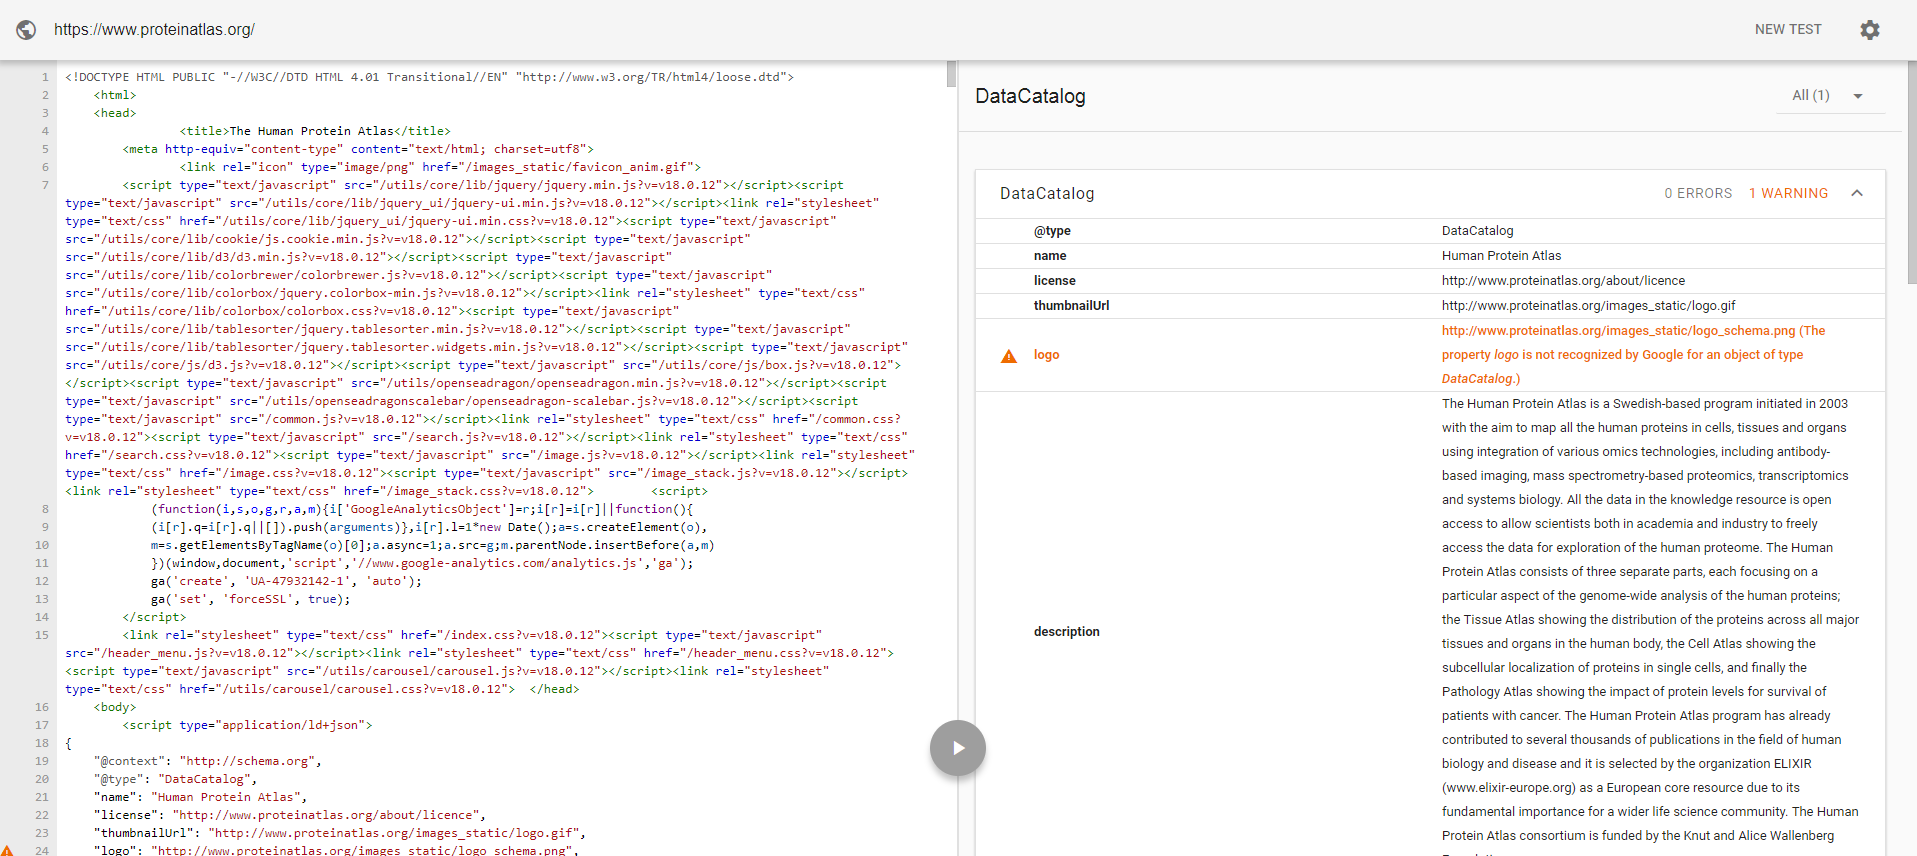
\includegraphics[scale=0.35]{images/google_testing.PNG}
   \caption{Google Structured Data Testing Tool}
   \label{fig:googleTool}
\end{figure}

\newpage
\subsubsection*{Validata}
Validata \footnote{\url{http://hw-swel.github.io/Validata/}(accessed 03/11/2018)} shown in Figure \ref{fig:validata} is a tool for "validating a RDF document against a set of constraints"\cite{hansen2015validata}. Constraints are expressed as a Shape Expression (ShEx) schema \cite{validataAG}. The user can select a schema that they would like their data to be validated against, currently supported schemas are Open PHACTS Dataset Description, HCLS Community Profile, DCAT or custom schema. The user then supplies either through a file or input box and then provides the results of the validation. Although not yet supported, this tool will eventually allow users to validate their JSON-LD against a description, providing another method for users to validate their Schema.org / Bioschemas markups.\newline

\begin{figure}[h]
 \centering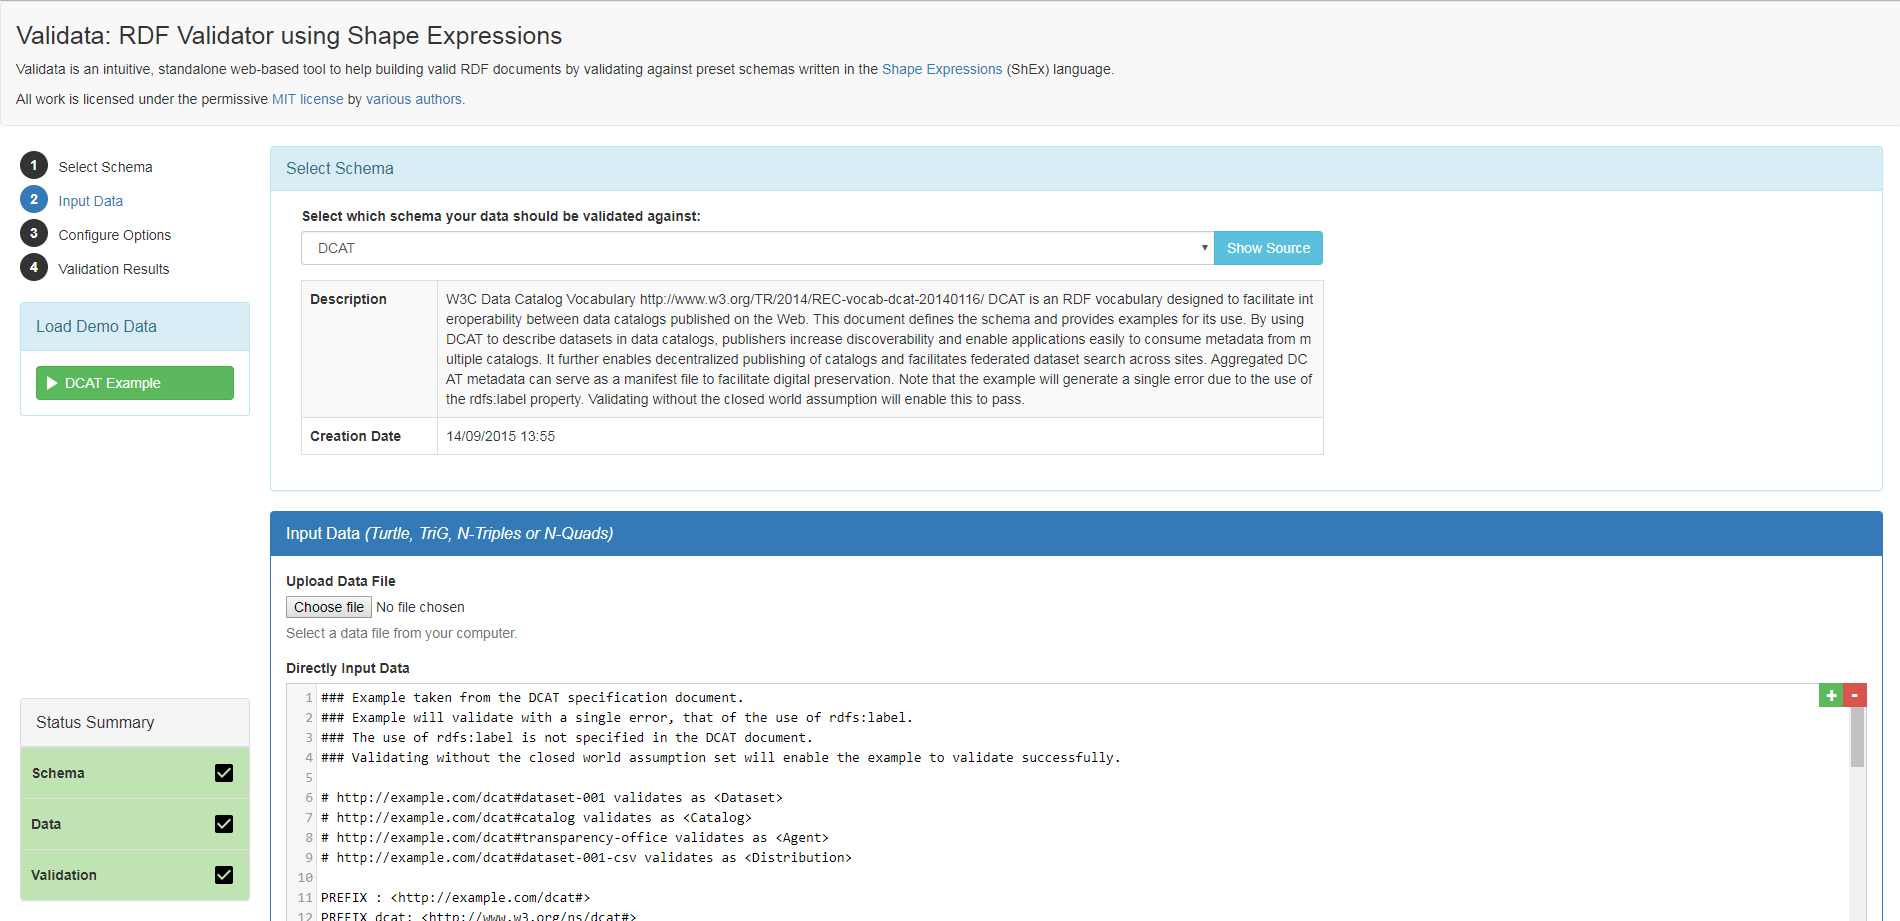
\includegraphics[scale=0.35]{images/validata.PNG}
   \caption{Validata: RDF Validator}
   \label{fig:validata}
\end{figure}

\newpage 
\section{Summary}
In conclusion, this chapter has examined Machine-readable data, more specifically the number of formats that are currently available for use on the web. Shown is the rise in use of machine-readable data on the web from webmasters, as large companies like Google and Bing have begun to provide tools and services to warrant their use.

Schema.org was covered, describing their solution to the vast amount of vocabularies for machine-readable data on the web by provide a single shared markup vocabulary. Due to the large number of properties and types available, webmasters struggle to choose decide which properties and types to best describe their web pages. Bioschemas.org Profiles and Google Dataset Search were discussed as a solution to this issue, as they research and recommend the most useful types and properties to include.

Finally, existing tools that aided in the generation and validation of Schema.org markup's were given and discussed. This is due to the proposed system having similar features to current Schema.org markup generators, and having a system to validate the data being produced will be vital.


